\documentclass[10pt]{article}
\usepackage[letterpaper,margin=2.2cm]{geometry}
\usepackage{mathptmx}
\usepackage{graphicx}
\usepackage{booktabs}
\usepackage{array}
\usepackage{caption}
\usepackage{float}
\usepackage{url}
\usepackage[hidelinks]{hyperref}
\newcolumntype{L}[1]{>{\raggedright\arraybackslash\hspace{0pt}}p{#1}}
\captionsetup{font=small,labelfont=bf}
\renewcommand{\thetable}{S\arabic{table}}
\renewcommand{\thefigure}{S\arabic{figure}}
\newcommand{\REO}{REO}
\newcommand{\ECRE}{EC-RE}
\newcommand{\Snap}{\Gamma}
\newcommand{\Trace}{\mathsf{T}}
\newcommand{\ArtSecReo}{IV-E}
\newcommand{\ArtSecExtension}{IV-D}
\newcommand{\ArtSecEvaluation}{VIII}
\newcommand{\ArtSecContract}{VIII-D}
\newcommand{\ArtSecImpact}{VIII-E}
\newcommand{\ArtAppRepro}{A}
\newcommand{\ArtTabFeatures}{2}
\newcommand{\ArtTabImpact}{10}
\newcommand{\ArtSecEvalDesign}{VIII-A}
\newcommand{\ArtPropSufficiency}{2}
\newcommand{\ArtSecViews}{IV-B}
\newcommand{\ArtSecShacl}{VIII-D4}
\newcommand{\ArtDefEnv}{2}
\newcommand{\ArtDefSlice}{3}
\newcommand{\ArtSecCandidates}{V-A}
\newcommand{\ArtSecObligations}{V-B}
\newcommand{\ArtSecPolicy}{V-D}
\newcommand{\ArtSecTrace}{VI-A}
\newcommand{\ArtSecSelection}{VI-B}
\newcommand{\ArtLstAnnotation}{1}

\makeatletter\def\rows#1{\@@input #1 }\makeatother
\setlength{\parskip}{3pt}
\setlength{\parindent}{0pt}

\title{Supplementary Material\\[4pt]\large Environment Engineering for Requirements Engineering:\\ The REO Ontology and an Executable Derivation Contract}
\author{Nihal Salih, Mohamed Amine El Youssr, Tarik Fissaa, and Mahmoud El Hamlaoui}
\date{Replication package of \REO{} v1.0.0 (contract policy \texttt{ecre-policy-1.0.0})}

\begin{document}
\maketitle

\section*{About this document}
This document holds the vocabulary tables, the detailed evaluation tables, and the terms and notation that the article cites as Fig.~S1, Tables~S1--S7, and Tables~S10--S12, a summary of the evidence per research question (Table~S8), and the version of every component of the replication package (Table~S9). Tables~S1--S6, S10, and S12 are written from the files that the pipeline of the replication package generates (\texttt{generated/*.tex}, \texttt{results/*.json}); no number in them was typed by hand. Section and table numbers without the prefix S refer to the article.

\begin{center}
\textbf{Contents of this document and the article sections they support}\\[4pt]
\small
\begin{tabular}{@{}lL{8.2cm}l@{}}
\toprule
\textbf{Item} & \textbf{Content} & \textbf{Article} \\
\midrule
Fig.~S1 & \REO{} v1.0.0 derivation module & Section \ArtSecReo \\
Table~S1 & The 37 object properties of \REO{} v1.0.0 & Section \ArtSecReo \\
Table~S2 & The 47 datatype properties of \REO{} v1.0.0 & Section \ArtSecReo \\
Table~S3 & Study E1: test suites written by language models without access to the code & Section \ArtSecContract \\
Table~S4 & Study E2: hand application of the contract by language-model analysts, per run & Section \ArtSecContract \\
Table~S5 & Element-level trace precision and recall, with the full threshold grid of text-similarity trace selection & Section \ArtSecImpact \\
Table~S6 & Identity migration: rename, split, and merge & Section \ArtSecImpact \\
Table~S7 & Coverage of the seven views by alternative metamodels & Section \ArtSecExtension \\
Table~S8 & Evidence and answers per research question & Section \ArtSecEvaluation \\
Table~S9 & Versions of the components of the replication package & Appendix \ArtAppRepro \\
Table~S10 & Mutation operators of the corpus & Section \ArtSecEvalDesign \\
Table~S11 & Terms and notation, with their values for requirement R001 & Section \ArtSecViews \\
Table~S12 & Schema-only validation versus contract decisions (confusion matrices) & Section \ArtSecShacl \\
\bottomrule
\end{tabular}
\end{center}

\section*{S1. The REO vocabulary}

\begin{figure}[H]
\centering
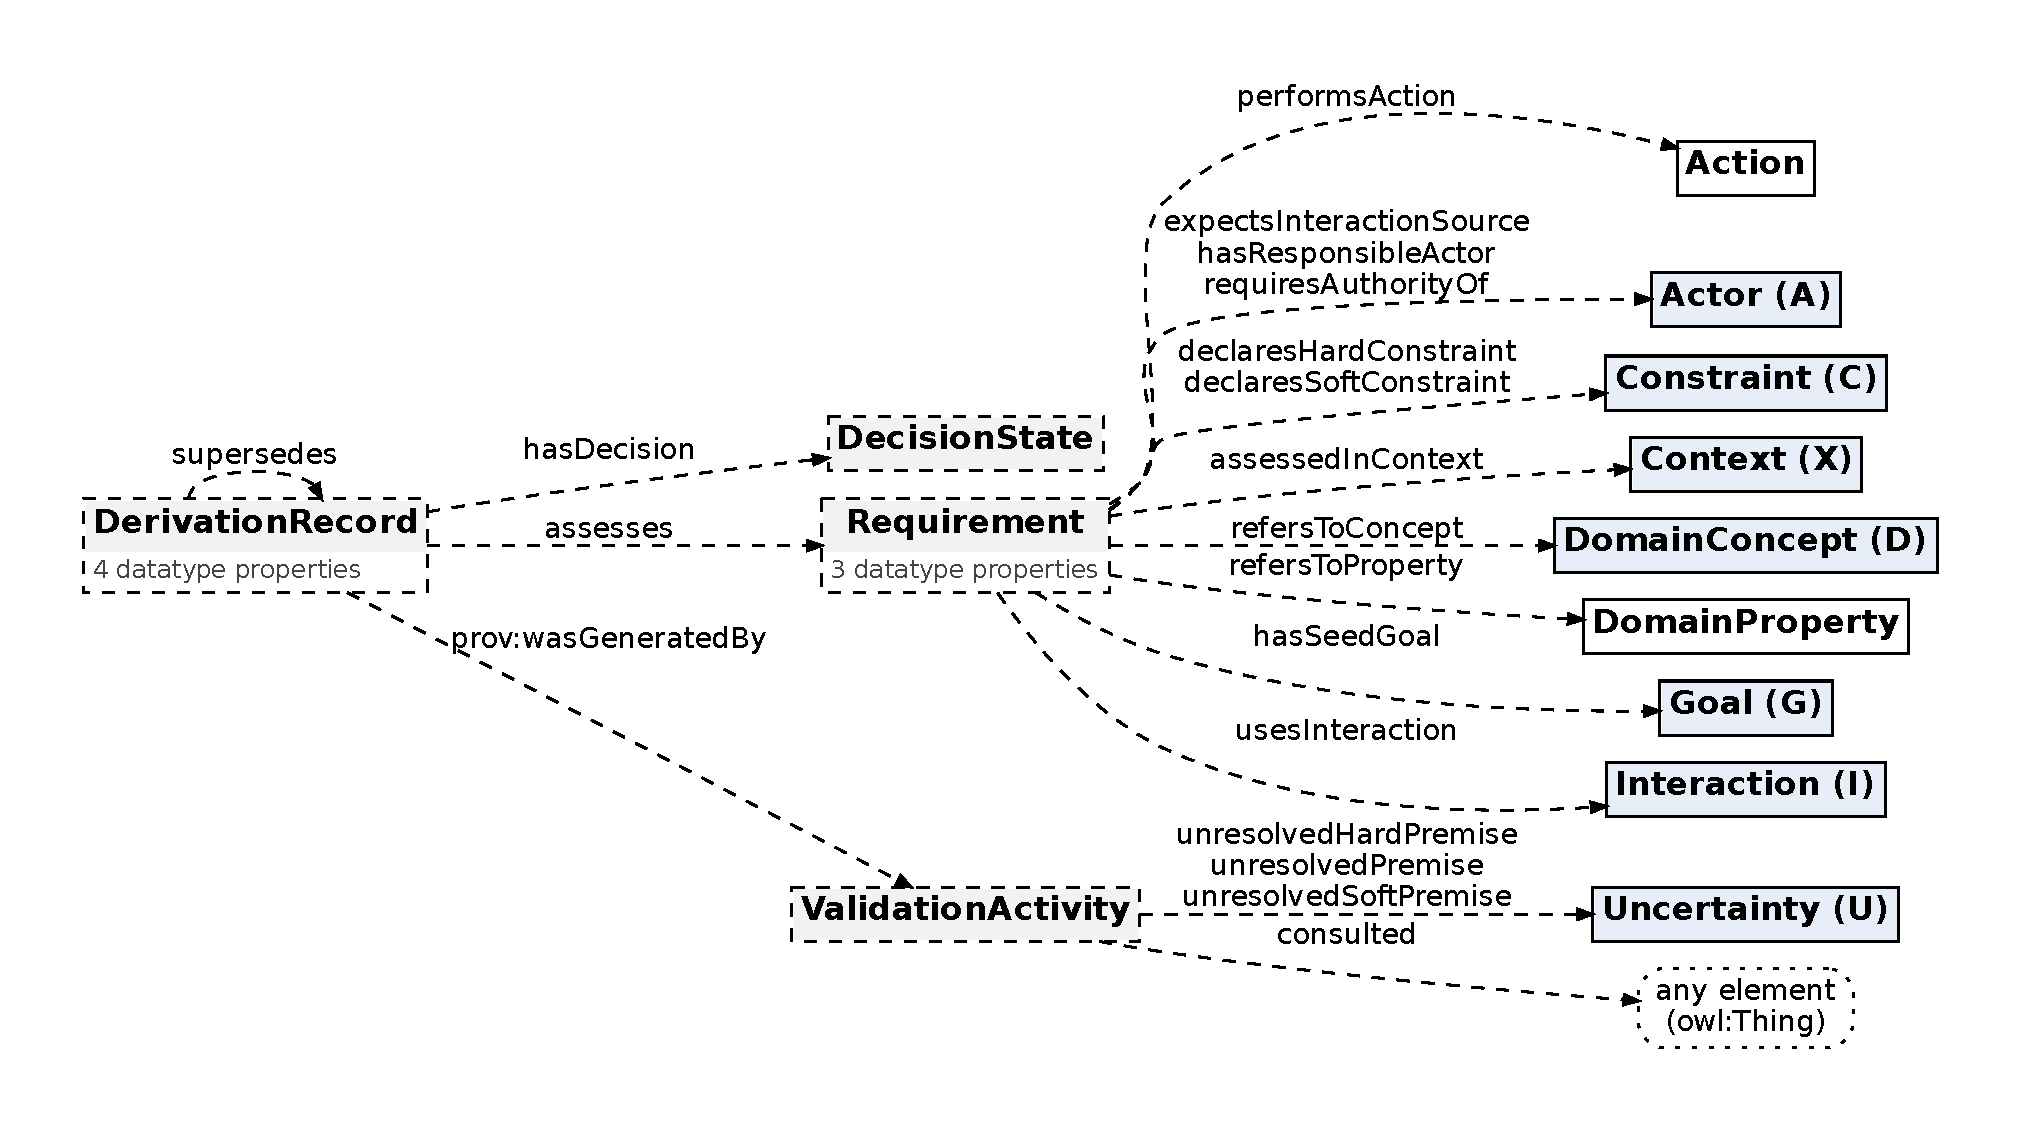
\includegraphics[width=\textwidth]{inputs/reo-derivation.pdf}
\caption{\REO{} v1.0.0 derivation module (dashed), generated from \texttt{reo-derivation.ttl} by \texttt{scripts/draw\_ontology.py}. Annotation links connect a \texttt{Requirement} to core classes. A \texttt{DerivationRecord} (a \texttt{prov:Entity}) assesses a requirement, has one \texttt{DecisionState}, and was generated by a \texttt{ValidationActivity} (a \texttt{prov:Activity}) that \texttt{consulted} the trace elements; \texttt{unresolvedHardPremise} and \texttt{unresolvedSoftPremise}, sub-properties of \texttt{unresolvedPremise}, mark the consulted uncertainties that the assessment did not establish, with their level.}
\end{figure}

\begin{table}[H]
\caption{The 37 object properties of \REO{} v1.0.0: subject class (domain), predicate, object class (range), and module. The derivation module also declares the reused PROV-O properties \texttt{prov:used} (specialized by \texttt{consulted}) and \texttt{prov:wasGeneratedBy}, which links a record to its validation activity; they are not counted.}
\small
\centering
\begin{tabular}{@{}llll@{}}
\toprule
\textbf{Domain} & \textbf{Predicate} & \textbf{Range} & \textbf{Module} \\
\midrule
\rows{inputs/tab_objprops.tex}
\bottomrule
\end{tabular}
\end{table}

\begin{table}[H]
\caption{The 47 datatype properties of \REO{} v1.0.0 by domain (range \texttt{xsd:string} unless stated). The derivation module also declares the reused \texttt{prov:startedAtTime}, which is not counted.}
\small
\begin{tabular}{@{}L{4.0cm}L{12.4cm}@{}}
\toprule
\textbf{Domain (count)} & \textbf{Properties} \\
\midrule
\rows{inputs/tab_dataprops.tex}
\bottomrule
\end{tabular}
\end{table}

\clearpage
\section*{S2. Detailed evaluation tables}

\begin{table}[H]
\caption{Study E1: test suites written by three language models (one author per model) from the specification pack, without access to the code. Scenarios; new requirements; expected decisions, of which non-trivial (different from the unmodified decision, or for a new requirement); expectations met before and after the runner correction (Section \ArtSecContract); competency questions answered as frozen.}
\small
\centering
\begin{tabular}{@{}llrrrrrrr@{}}
\toprule
\textbf{Author} & \textbf{Model} & \textbf{Scen.} & \textbf{New req.} & \textbf{Exp.} & \textbf{Non-triv.} & \textbf{Before} & \textbf{After} & \textbf{CQ} \\
\midrule
\rows{inputs/tab_llm_e1.tex}
\midrule
Total & & 36 & 25 & 385 & 112 & 384 & 385 & 24/24 \\
\bottomrule
\end{tabular}
\end{table}

\begin{table}[H]
\caption{Study E2: language-model analysts applying the contract by hand to 20 mutants sampled by operator (seed 2026), 200 decisions per run. DOC: prose description generated from the Turtle; MODEL: \REO{} files and triple changes, without the checker. Correct decisions; precision (P) and recall (R) of the changed decisions (25 in the sample); mutants without any error; seconds per decision. The reference is the checker's decision, confirmed by the SPARQL encoding on every pair.}
\small
\centering
\begin{tabular}{@{}llcccccc@{}}
\toprule
\textbf{Condition} & \textbf{Model} & \textbf{Run} & \textbf{Correct} & \textbf{P} & \textbf{R} & \textbf{Mutants without error} & \textbf{s/decision} \\
\midrule
\rows{inputs/tab_llm_e2.tex}
\bottomrule
\end{tabular}
\end{table}

\begin{table}[H]
\caption{Element-level trace precision (P), recall (R), and F1 against behavior-derived relevance (unit: a requirement--element pair; 96 relevant pairs), and, for text-similarity trace selection, the share of the 1,197 changed assessments that its impact selection misses and its cost (mean requirements reassessed per change, of ten) at each threshold $\tau$ of the grid. The best threshold, $\tau=0.05$, is selected on the test data and is therefore optimistic. The impact selection of the read-set and view-level traces is reported in Table~\ArtTabImpact{} of the article.}
\small
\centering
\begin{tabular}{@{}lcccccc@{}}
\toprule
\textbf{Trace} & $\tau$ & \textbf{P} & \textbf{R} & \textbf{F1} & \textbf{Impact miss rate} & \textbf{Cost} \\
\midrule
\rows{inputs/tab_trace_grid.tex}
\bottomrule
\end{tabular}
\end{table}

\begin{table}[H]
\caption{Identity migration on three successor snapshots, for the ten requirements and the test requirement R011. Selected: requirements selected by trace-based selection; migrated: requirements whose references are rewritten; missed: migrated requirements not selected; naive: decisions changed by naive reassessment, which ignores identity; preserved: decisions preserved by identity-aware reassessment; ambiguous: references sent to review.}
\small
\centering
\begin{tabular}{@{}L{5.6cm}cccccc@{}}
\toprule
\textbf{Change} & \textbf{Selected} & \textbf{Migrated} & \textbf{Missed} & \textbf{Naive} & \textbf{Preserved} & \textbf{Ambiguous} \\
\midrule
\rows{inputs/tab_migration.tex}
\bottomrule
\end{tabular}
\end{table}

\begin{table}[H]
\caption{Coverage of the seven views by alternative metamodels (from Table~\ArtTabFeatures{} of the article: first-class; partial) and their constructs without a \REO{} counterpart.}
\small
\centering
\begin{tabular}{@{}L{3.0cm}L{4.4cm}L{7.6cm}@{}}
\toprule
\textbf{Metamodel} & \textbf{Views: first-class; partial} & \textbf{Not represented in \REO} \\
\midrule
KAOS & A, G, D, U; C, I & obstacle refinement, goal semantics in linear temporal logic \\
iStar 2.0 & A, G, I; -- & contribution links, softgoal evaluation \\
CORE ontology & G, D, C; -- & attitudes, preference evaluation \\
SysML v2 requirements & A, D, C, I; G, U & verification cases, behavior \\
\bottomrule
\end{tabular}
\end{table}

\clearpage
\section*{S3. Evidence summary and versions}

\begin{table}[H]
\caption{Evidence and answers per research question (Section \ArtSecEvaluation{} of the article). All results are artifact-level: they concern the implementation, its agreement with a second encoding and with readings of the specification, and a synthetic model; none comes from human participants.}
\small
\begin{tabular}{@{}L{0.9cm}L{5.2cm}L{10.2cm}@{}}
\toprule
\textbf{RQ} & \textbf{Evidence} & \textbf{Answer} \\
\midrule
RQ1 & Retrospective coding of 12 frameworks against 17 concerns; two codings by language models (E3, sensitivity check); views of the 96 behavior-derived relevant pairs & The four criteria retain the seven views under the reference coding; six views are retained under all three codings, and uncertainty is kept for its role in the decision. In the example, every view feeds some decision, and each decision depends on five to seven views. A consistency check, not an independent validation; bounded to the decision task. \\
RQ2 & HermiT with 8 injected errors; SHACL fixtures; pitfall scan; 34 competency questions & Consistent, with no unsatisfiable class; all 8 errors detected; no pitfall except one informative finding; 34 of 34 answers as expected. \\
RQ3 & 38 regression cases and 4 impact queries; 779 mutants (7,790 assessments) with differential testing; E1 (385 expectations); E2 (8 runs of 200 decisions); two decision rules derived from SHACL alone; 68 corner cases; 561 annotation perturbations & All expected states; 7,790 of 7,790 assessments agree between the two implementations; 385 of 385 expectations met once the test runner migrates references (384 in the first execution); 199 or 200 of 200 hand decisions correct per run, without a trace; schema-only verdicts agree with the decisions on 22.5\% and 36.1\% of the assessments. \REO{} v1.0.0 passes 68 of 68 corner cases; the premise-removal rule changes 4 of the 7,790 corpus decisions. For acceptance-type requirements, 52\% of the single-field annotation errors become visible and 42\% leave the decision unchanged; 12 of 561 perturbations make a decision more permissive. \\
RQ4 & Behavior-derived relevance (96 requirement--element pairs); seven selection rules over 779 mutants (7,790 mutant--requirement pairs); three identity-migration cases; property checks V1--V4 (5,000 random mutants, 200 vocabulary edits, 38 renames, 5,000 pairs of random snapshots) & Read-set traces: element-level precision 0.88, recall 1.00. With the touched-identifier diff, impact selection misses none of the 1,197 changed assessments (recall 1.00; precision 0.28 at the assessment level and 0.16 at the decision level) while reassessing 5.50 of ten requirements per change; coarser rules miss 29\% to 34\%, text similarity 43\% to 83\%. No violation of Proposition~\ArtPropSufficiency{} was observed in V1 and V4; V2 selects all 376 changed decisions; V3 reproduces the 380 decisions of direct substitution. One-step migration preserves 11 of 11 decisions under rename and merge, and 10 of 11 under the split, which sends one ambiguous reference to review. \\
\bottomrule
\end{tabular}
\end{table}

\begin{table}[H]
\caption{Versions of the components of the replication package of REO v1.0.0, read from the files (\texttt{supplement/make\_inputs.py}).}
\small
\begin{tabular}{@{}L{5.0cm}L{3.6cm}L{7.6cm}@{}}
\toprule
\textbf{Component} & \textbf{Version} & \textbf{Note} \\
\midrule
Replication package & REO v1.0.0 & \texttt{CITATION.cff}, \texttt{CHANGELOG.md}; to be deposited on Zenodo with a version DOI (not yet deposited) \\
Core ontology \texttt{reo-core.ttl} & 1.0.0 & version IRI \url{http://re-environment-onto.org/ontology/release/1.0.0} \\
Derivation module \texttt{reo-derivation.ttl} & 1.0.0 & version IRI \url{http://re-environment-onto.org/ontology/derivation/release/1.0.0} \\
Core shapes \texttt{reo-shapes.ttl} & no version label in the file & validated with the ontology modules and RDFS inference \\
Derivation shapes \texttt{reo-derivation-shapes.ttl} & REO v1.0.0 & record history and annotation well-formedness shapes \\
Reference checker \texttt{reo\_checker.py} & REO v1.0.0 & implements policy \texttt{ecre-policy-1.0.0} \\
SPARQL encoding \texttt{sparql\_oracle.py} & REO v1.0.0 & implements policy \texttt{ecre-policy-1.0.0} \\
Contract policy & \texttt{ecre-policy-1.0.0} & written into every decision record (\texttt{reo:policyVersion}) \\
Evaluation scripts & REO v1.0.0 & \texttt{scripts/run\_all.py} (25 steps); run manifest of 2026-11-10 \\
Example and fixtures & labelled REO v1.0.0 & synthetic medical-emergency example, extension, ten requirements, three SHACL fixtures \\
Competency-question suite & cq\_suite.json & 34 questions \\
Language-model study packs & frozen before the studies & specification packs and outputs of E1--E3, frozen and hashed before execution; the derivation module of the pack lacks 4 properties of decision records (\texttt{candidateSnapshot}, \texttt{unresolvedHardPremise}, \texttt{unresolvedPremise}, \texttt{unresolvedSoftPremise}), which the studies do not use; the example files are identical \\
Software of the recorded run & Python 3.13.18 & RDFLib 7.6.0, pySHACL 0.40.0, Owlready2 0.51, OpenJDK 21 \\
\bottomrule
\end{tabular}
\end{table}


\clearpage
\section*{S4. Mutation corpus}

\begin{table}[H]
\caption{Mutation operators of the corpus (Section \ArtSecEvalDesign{} of the article), number of mutants, and number of mutants that change at least one of the ten decisions.}
\small
\centering
\begin{tabular}{@{}lL{7.0cm}rr@{}}
\toprule
\textbf{Operator} & \textbf{Change} & \textbf{Mutants} & \textbf{Changing} \\
\midrule
\rows{inputs/tab_operators.tex}
\midrule
\rows{inputs/tab_operators_total.tex}
\bottomrule
\end{tabular}
\end{table}

\section*{S5. Terms and notation; schema-only validation}

\begin{table}[H]
\caption{Terms and notation of the article, with their value for requirement R001 of the example.}
\scriptsize
\begin{tabular}{@{}L{3.6cm}L{8.9cm}L{3.6cm}@{}}
\toprule
\textbf{Term} & \textbf{Meaning} & \textbf{For R001} \\
\midrule
Environment snapshot $\Snap_t$ & The model at version $t$ (Definition~\ArtDefEnv{} of the article) as an RDF graph, without annotations or records. & base model and extension \\
Seed slice $S_0$ & Conceptual input of candidate production (Definition~\ArtDefSlice); not used by the contract. & not computed \\
Candidate $q$, annotation $\alpha(q)$ & A sentence and the RDF triples that map it to model elements (Section~\ArtSecCandidates). & R001; Listing~\ArtLstAnnotation{} \\
Seed goal $g$, lineage $L(g)$; context $x$ & The goal served, with the goals it refines directly or indirectly; the situation assessed. & G002; $\{$G002, G001$\}$; X001 \\
References $\mathit{refs}(q)$ & Responsible actor, authority holder, actions, concepts, properties, interaction, expected source. & 8 elements (Listing~\ArtLstAnnotation) \\
Applicable constraints $R(q)$ & The rules that apply to $q$ through one of five routes (Section~\ArtSecObligations). & C001, C002, C003 \\
Evidence $E(q)$ & $\mathit{refs}(q)\cup L(g)\cup R(q)\cup\{x\}$: what the checks read; specific to $q$, distinct from $S_0$. & 14 elements \\
Obligation instance $\omega$, level $\ell(\omega)$, outcome $r(\omega)$ & A check of kind O1--O9 on one element (Section~\ArtSecObligations); hard or soft; \emph{pass}, \emph{fail}, \emph{unchecked} (undecidable with the model and validators), \emph{not triggered}, or \emph{open} (premise not yet verified). & O8 for U001: hard, open \\
Decision state; justifications $J$ & One of six states chosen by ordered rules (Section~\ArtSecPolicy); the outcomes with their messages. & \textit{conditional}; 13 entries \\
Trace $\Trace_q$ (read set) & Every element that the decision read (Section~\ArtSecTrace). & 15 elements \\
Touched identifiers $\Delta$; trace-based selection & Elements that an added or removed triple is about or points to; reassessing the requirements whose trace meets $\Delta$ (Section~\ArtSecSelection). & $\{$U001$\}$ selects R001, R007 \\
\bottomrule
\end{tabular}
\end{table}

\begin{table}[H]
\caption{Schema-only validation (Section~\ArtSecShacl{} of the article): verdicts of the global and the requirement-focused SHACL decision rules (rows) versus contract decisions (columns) over the 7,790 assessments of the corpus. acc: accepted; res: accepted with reservations; cond: conditional; rev: pending review; rej: rejected; n/d: not derived. A SHACL accept counts as agreeing with acc and res.}
\small
\centering
\begin{tabular}{@{}llrrrrrr@{}}
\toprule
\textbf{Rule} & \textbf{SHACL verdict} & \textbf{acc} & \textbf{res} & \textbf{cond} & \textbf{rev} & \textbf{rej} & \textbf{n/d} \\
\midrule
\rows{inputs/tab_shacl_confusion.tex}
\bottomrule
\end{tabular}
\end{table}

\end{document}
